% Options for packages loaded elsewhere
\PassOptionsToPackage{unicode}{hyperref}
\PassOptionsToPackage{hyphens}{url}
%
\documentclass[
]{article}
\usepackage{amsmath,amssymb}
\usepackage{lmodern}
\usepackage{iftex}
\ifPDFTeX
  \usepackage[T1]{fontenc}
  \usepackage[utf8]{inputenc}
  \usepackage{textcomp} % provide euro and other symbols
\else % if luatex or xetex
  \usepackage{unicode-math}
  \defaultfontfeatures{Scale=MatchLowercase}
  \defaultfontfeatures[\rmfamily]{Ligatures=TeX,Scale=1}
\fi
% Use upquote if available, for straight quotes in verbatim environments
\IfFileExists{upquote.sty}{\usepackage{upquote}}{}
\IfFileExists{microtype.sty}{% use microtype if available
  \usepackage[]{microtype}
  \UseMicrotypeSet[protrusion]{basicmath} % disable protrusion for tt fonts
}{}
\makeatletter
\@ifundefined{KOMAClassName}{% if non-KOMA class
  \IfFileExists{parskip.sty}{%
    \usepackage{parskip}
  }{% else
    \setlength{\parindent}{0pt}
    \setlength{\parskip}{6pt plus 2pt minus 1pt}}
}{% if KOMA class
  \KOMAoptions{parskip=half}}
\makeatother
\usepackage{xcolor}
\IfFileExists{xurl.sty}{\usepackage{xurl}}{} % add URL line breaks if available
\IfFileExists{bookmark.sty}{\usepackage{bookmark}}{\usepackage{hyperref}}
\hypersetup{
  hidelinks,
  pdfcreator={LaTeX via pandoc}}
\urlstyle{same} % disable monospaced font for URLs
\usepackage{longtable,booktabs,array}
\usepackage{calc} % for calculating minipage widths
% Correct order of tables after \paragraph or \subparagraph
\usepackage{etoolbox}
\makeatletter
\patchcmd\longtable{\par}{\if@noskipsec\mbox{}\fi\par}{}{}
\makeatother
% Allow footnotes in longtable head/foot
\IfFileExists{footnotehyper.sty}{\usepackage{footnotehyper}}{\usepackage{footnote}}
\makesavenoteenv{longtable}
\usepackage{graphicx}
\makeatletter
\def\maxwidth{\ifdim\Gin@nat@width>\linewidth\linewidth\else\Gin@nat@width\fi}
\def\maxheight{\ifdim\Gin@nat@height>\textheight\textheight\else\Gin@nat@height\fi}
\makeatother
% Scale images if necessary, so that they will not overflow the page
% margins by default, and it is still possible to overwrite the defaults
% using explicit options in \includegraphics[width, height, ...]{}
\setkeys{Gin}{width=\maxwidth,height=\maxheight,keepaspectratio}
% Set default figure placement to htbp
\makeatletter
\def\fps@figure{htbp}
\makeatother
\setlength{\emergencystretch}{3em} % prevent overfull lines
\providecommand{\tightlist}{%
  \setlength{\itemsep}{0pt}\setlength{\parskip}{0pt}}
\setcounter{secnumdepth}{-\maxdimen} % remove section numbering
\makeatletter
\@ifpackageloaded{subfig}{}{\usepackage{subfig}}
\@ifpackageloaded{caption}{}{\usepackage{caption}}
\captionsetup[subfloat]{margin=0.5em}
\AtBeginDocument{%
\renewcommand*\figurename{Figure}
\renewcommand*\tablename{Table}
}
\AtBeginDocument{%
\renewcommand*\listfigurename{List of Figures}
\renewcommand*\listtablename{List of Tables}
}
\newcounter{pandoccrossref@subfigures@footnote@counter}
\newenvironment{pandoccrossrefsubfigures}{%
\setcounter{pandoccrossref@subfigures@footnote@counter}{0}
\begin{figure}\centering%
\gdef\global@pandoccrossref@subfigures@footnotes{}%
\DeclareRobustCommand{\footnote}[1]{\footnotemark%
\stepcounter{pandoccrossref@subfigures@footnote@counter}%
\ifx\global@pandoccrossref@subfigures@footnotes\empty%
\gdef\global@pandoccrossref@subfigures@footnotes{{##1}}%
\else%
\g@addto@macro\global@pandoccrossref@subfigures@footnotes{, {##1}}%
\fi}}%
{\end{figure}%
\addtocounter{footnote}{-\value{pandoccrossref@subfigures@footnote@counter}}
\@for\f:=\global@pandoccrossref@subfigures@footnotes\do{\stepcounter{footnote}\footnotetext{\f}}%
\gdef\global@pandoccrossref@subfigures@footnotes{}}
\@ifpackageloaded{float}{}{\usepackage{float}}
\floatstyle{ruled}
\@ifundefined{c@chapter}{\newfloat{codelisting}{h}{lop}}{\newfloat{codelisting}{h}{lop}[chapter]}
\floatname{codelisting}{Listing}
\newcommand*\listoflistings{\listof{codelisting}{List of Listings}}
\makeatother
\ifLuaTeX
  \usepackage{selnolig}  % disable illegal ligatures
\fi
\usepackage[]{natbib}
\bibliographystyle{plainnat}

\author{}
\date{}

\begin{document}

The Interfaces usability is evaluated with an exemplary implementation
of a non-trivial scheduling algorithm. Since the Interfaces can manage
multiple Testbeds inside the same cluster, a Profiling-Scheduler
approach is chosen to highlight some of the interface's features.

The example scheduling algorithm is used on a 5 Node cluster running
inside the Google Cloud Platforms Kubernetes Engine (GKE). During
development, smaller Nodes with a single vCPU and 4Gi of Memory were
sufficient, but for the final evaluation, Nodes were doubled in
capacity.

\begin{figure}
\centering
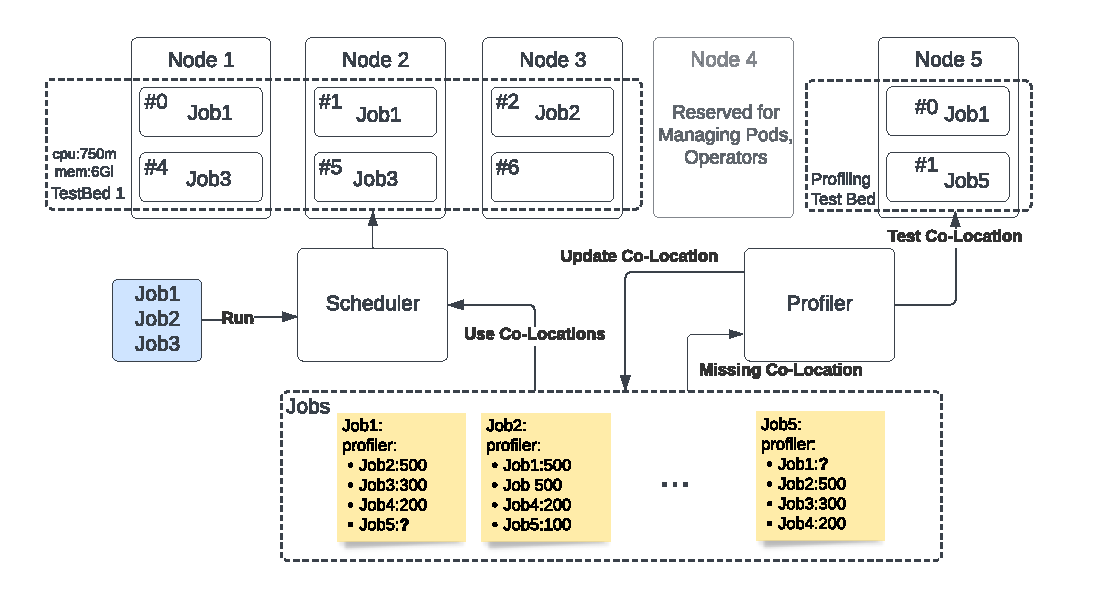
\includegraphics{graphics/evaluation_example_scheduler_arch.pdf}
\caption{Architecture of the Example Profiler-Scheduler}
\end{figure}

Two Test-Beds are created using the Test-Bed CRD, the Profiling Testbed,
and the Testbed for the actual execution of Jobs. The slot size was
chosen depending on the resources available. For the final evaluation, a
slot size of 750m CPU and 3Gi Memory leaves enough resources available
for the cluster's control plane, managing Pods (Driver, JobManager), and
the Operators running inside the cluster.

Contrary to the Scheduler Thread, which only creates a scheduling if
requested (via stdin), the Profiler Thread runs at all times, updating
and refining the Co-Location Matrix by choosing job pairings with the
least data points. To test the systems stability the scheduling thread
was later modified to create schedulings by choosing jobs at random.

Co-Locations are described as a simple runtime in seconds. By iterating
over the available job pairings, the Profiler builds a Co-Location
Matrix. The Profiler creates a cumulative moving average for each job
pairing.

Jobs cannot be paired with themself since the acquire/release mechanism
only allows a single execution per job at a time. In theory, Jobs can be
Co-Located with itself by deploying the application with a replication
of two, but this could not be directly compared to Co-Location with a
different job, as work done is split between both instances.

\begin{longtable}[]{@{}
  >{\raggedleft\arraybackslash}p{(\columnwidth - 10\tabcolsep) * \real{0.1717}}
  >{\centering\arraybackslash}p{(\columnwidth - 10\tabcolsep) * \real{0.1616}}
  >{\centering\arraybackslash}p{(\columnwidth - 10\tabcolsep) * \real{0.1616}}
  >{\centering\arraybackslash}p{(\columnwidth - 10\tabcolsep) * \real{0.1818}}
  >{\centering\arraybackslash}p{(\columnwidth - 10\tabcolsep) * \real{0.1717}}
  >{\centering\arraybackslash}p{(\columnwidth - 10\tabcolsep) * \real{0.1515}}@{}}
\toprule
\begin{minipage}[b]{\linewidth}\raggedleft
\end{minipage} & \begin{minipage}[b]{\linewidth}\centering
batchjob-flink
\end{minipage} & \begin{minipage}[b]{\linewidth}\centering
batchjob-spark
\end{minipage} & \begin{minipage}[b]{\linewidth}\centering
batchjob-sample3
\end{minipage} & \begin{minipage}[b]{\linewidth}\centering
batchjob-flink2
\end{minipage} & \begin{minipage}[b]{\linewidth}\centering
spark-crawler
\end{minipage} \\
\midrule
\endhead
batchjob-flink & / & 36 (5) & 28 (11) & 24 (16) & 34 (11) \\
batchjob-spark & 70 (4) & / & 93 (4) & 68 (4) & 94 (4) \\
batchjob-sample3 & 444 (4) & 480 (6) & / & 450 (3) & 493 (3) \\
batchjob-flink2 & 24 (16) & 36 (5) & 30 (11) & / & 25 (10) \\
spark-crawler & 173 (3) & 203 (5) & 211 (3) & 171 (3) & / \\
\bottomrule
\end{longtable}

\textbf{Note:} The matrix is not symmetrical because the runtime of each
job is used, not the runtime of both jobs (or the runtime of the
complete scheduling). The runtime of the scheduling is the time after
acquisition until all jobs have been completed. The Batch Job Operator
only tracks the application's time inside the running state. This
approach was chosen because applications may have vastly different
startup times, which will become insignificant for long-running jobs.

The Scheduling Thread is the traditional scheduler. Given a list of
Jobs, the Scheduling Thread tries to find optimal scheduling regarding
total runtime. The scheduler takes a greedy approach choosing the
co-located job based on the job with the shortest runtime to keep the
evaluation simple. Replication of each job is selected based on the
number of slots (Replication = NumberOfSlots / NumberOfJobs). Empty
slots are again greedily filled with jobs suited best for co-location,
not allowing a job to be chosen more than once.

Both the Profiler and the Scheduler run in parallel. If any of them
cannot acquire their jobs, the scheduling will wait until they become
available.

\end{document}
